\section{Prediktívne riadenie}
\label{se:teoriaMPC}

Prediktívne riadenie, pod anglickou skratkou MPC, je známe už od minulého storočia. Je jednou z najpoužívanejších foriem riadenia s optimalizáciou. Dokáže zvládať mnohorozmerné riadenie, jedna z jeho najväčších výhod je, že doň vieme zahrnúť ohraničenie. Tým poskytuje obrovskú prevahu oproti svojmu predchodcovi, lineárnemu kvadratickému regulátoru, inak LQR. 

Základnou myšlienkou MPC je, že pomocou známeho matematického modelu systému vieme predikovať budúce správanie sa procesu na pevne určenom časovom horizonte. Tieto informácie vieme využiť pri výpočte optimálnych akčných zásahov, pomocou minimalizácie účelovej funkcie. Takto navrhnuté riadenie nám zabezpečuje garanciu dodržania všetkých ohraničení.

\subsection{Formulácia MPC}
\label{subse:MPC}
Ako sme už spomínali v rámci MPC je nutné poznať matematický model reprezentujúci riadený systém, či už v lineárnej alebo nelineárnej podobe. Najčastejšie sa používa lineárny model v tvare diskrétnej stavovej rovnice v nasledovnej podobe
\begin{align}
	x_{k+1} = Ax_{k} + Bu_{k}\\
	y_{k} = Cx_{k} + Du_{k}
\end{align}
kde $x$ predstavuje stĺpcový vektor stavov o veľkosti $n_{x}$, $u$ predstavuje stĺpcový vektor vstupov o veľkosti $n_{u}$, $A$ je matica stavov definovaná ako $A \in {\rm I\!R}^{n_{x}\times n_{x}}$, B je matica vstupov definovaná ako $B \in {\rm I\!R}^{n_{u}\times n_{u}}$. Rovnicu (2.2), ktorá predstavuje rovnicu výstupu zo systému môžme pri návrhu MPC zanedbať, budeme totiž brať do úvahy iba stavové riadenie.

Základnú formuláciu lineárneho MPC si zadefinujeme nasledovne
\label{math:LinearneMPC}
\begin{subequations}
	\begin{align}
		\displaystyle \min_{u_0,...,u_{N-1}} \hspace{0.1cm} & 
		\sum_{k=1}^{N}\norm{Qx_k}^{2}_{2}+\sum_{k=0}^{N-1}\norm{Ru_k}^{2}_{2}\\
		\textrm{s.t.} \hspace{0.5cm} & x_{k+1} = Ax_{k}+Bu_{k}\hspace{0.5cm} k=0,\dots,N-1\\
		& x_{0} = x(t)\\
		& \underline{x} \leq x_{k} \leq \overline{x}\hspace{0.5cm} k=0,\dots,N\\
		& \underline{u} \leq u_{k} \leq \overline{u}\hspace{0.5cm} k=0,\dots,N-1
	\end{align}
\end{subequations}
kde matica $Q$ predstavuje váhovú maticu stavov definovanú ako $Q \in {\rm I\!R}^{n_{x}\times n_{x}}$, matica $R$ je váhová maticu vstupov definovaná ako $R \in {\rm I\!R}^{n_{u}\times n_{u}}$. Pomocou týchto váhových matíc si môžme nastavovať prioritu počas optimalizácie pre každý stav a vstup samostatne. 

\subsection{Lineárne riadenie s kompenzáciou nelinearity}
\label{subse:LinearneMPCKomp}
Najjednoduchšou formou prediktívneho riadenia je lineárne riadenie. V rámci MPC sa používa lineárny model s lineárnymi ohraničeniami. Ide o najmenej komplikovanú formu, ktorá má výhodu v krátkom výpočtovom čase, čo sa môže hodiť pri systémoch s rýchlou dynamikou. Keďže všetko je vždy o kompromisoch a za rýchlym výpočtovým časom je veľa zanedbaní, ktoré sú najmä v lineárnom modeli. V realite sa málokedy stretneme so systémom, ktorý by stačilo opísať jednoduchým stavovým modelom a riadenie by fungovalo bezchybne. 
\begin{figure}[H]
	\centering
	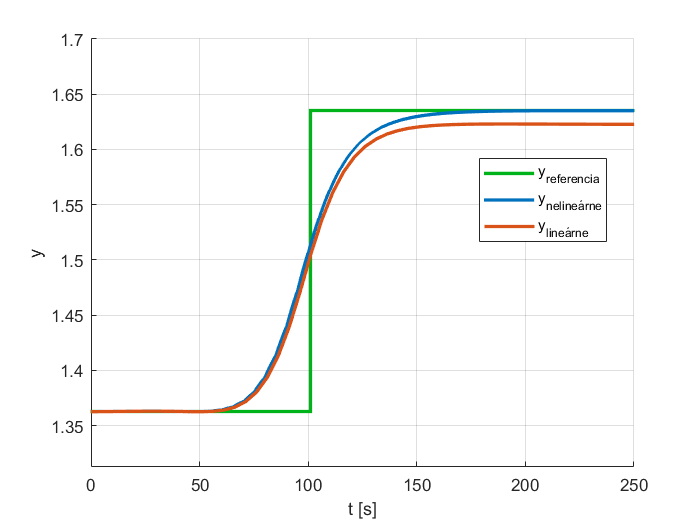
\includegraphics[width=11cm,height=8cm]{images/linear_vs_nonlinear}
	\caption{Rozdiel medzi lineárnim a nelineárnim riadením}
\end{figure}
Pri takomto riadení vznikajú trvalé regulačné odchýlky (Obr.2.1). Aby sa tomu predišlo, musia sa pridávať doplnkové opatrenia, ktoré by vyrovnávali nelinearitu. 

Jedným z najefektívnejších je pridať integračné vlastnosti regulátoru. Pomocou nich bude regulátor minimalizovať rozdiel medzi nelineárnym procesom a lineárnym modelom procesu. Jednoducho sa pridá do lineárneho modelu porucha, ktorá bude reprezentovať tento rozdiel. Takže rovnicu (2.1) nahradíme novým systémom, rozšíreným o poruchu.
\begin{align}
	x_{k+1} &= Ax_{k} + Bu_{k} + Ed_{k}\\
	d_{k+1} &= d_{k}
\end{align}
Nastáva problém, odkiaľ sa získajú aktuálne hodnoty poruchy, reprezentujúcej odchýlku od nelinearity. Takýto člen sa nedá priamo merať senzorom, dá sa ale získať pomocou odhadu. Môžeme využiť buď Luenbergerov pozorovateľ, alebo pokročilejší, časovo premenný Kalmanov filter. 

Výsledná forma takto zadefinovaného MPC bude v nasledovnom tvare.
\begin{subequations}
	\begin{align}
	\displaystyle \min_{u_0,...,u_{N-1}} \hspace{0.1cm} & 
	\sum_{k=1}^{N}\norm{Qx_k}^{2}_{2}+\sum_{k=0}^{N-1}\norm{Ru_k}^{2}_{2}\\
	\textrm{s.t.} \hspace{0.5cm} & x_{k+1} = Ax_{k} + Bu_{k} + E\hat{d}_{k}\hspace{0.5cm} k=0,\dots,N-1\\
	& x_{0} = x(t)\\
	& \hat{d}_{0} = \hat{d}(t)\\
	& \underline{x} \leq x_{k} \leq \overline{x}\hspace{0.5cm} k=0,\dots,N\\
	& \underline{u} \leq u_{k} \leq \overline{u}\hspace{0.5cm} k=0,\dots,N-1
	\end{align}
\end{subequations}
kde $\hat{d}$ predstavuje rozdiel medzi lineárnym a nelineárnym modelom systému, $E$ je jednotková matica definovaná ako $E \in {\rm I\!R}^{n_{x}\times n_{x}}$.

\subsection{Nelineárne riadenie}
\label{subse:NelinearneMPC}
Ak by sme chceli predísť všetkým prídavkom k lineárnemu riadeniu a následnému ladeniu všetkých pridaných váhových matíc, je možnosť priamo vymeniť lineárny model za nelineárny. V rámci tejto práce sa budeme venovať práve takémuto nelineárnemu riadeniu, tak, že nahradíme lineárny model používaný v MPC priamo za nelineárny.

Nelineárne rovnice budú vo forme diferenciálnych rovníc, ktoré následne diskretizujeme v rámci periódy vzorkovania systému. Takto získanú rovnicu použijeme miesto stavového opisu a výsledné MPC bude mať nasledovnú formu.
\begin{subequations}
	\begin{align}
	\displaystyle \min_{u_0,...,u_{N-1}} \hspace{0.1cm} & 
	\sum_{k=1}^{N}\norm{Qx_k}^{2}_{2}+\sum_{k=0}^{N-1}\norm{Ru_k}^{2}_{2}\\
	\textrm{s.t.} \hspace{0.5cm} & x_{k+1} = f(x_{k},u_{k},T_{s})\hspace{0.5cm} k=0,\dots,N-1\\
	& x_{0} = x(t)\\
	& \underline{x} \leq x_{k} \leq \overline{x}\hspace{0.5cm} k=0,\dots,N\\
	& \underline{u} \leq u_{k} \leq \overline{u}\hspace{0.5cm} k=0,\dots,N-1
	\end{align}
\end{subequations}
Takýto prístup môže spôsobiť komplikácie pri riešení MPC. Výrazne sa zväčší výpočtový čas a je komplikovanejšie s ním narábať. Cieľom tejto práce bude zrýchliť aj takéto riadenie tak, aby ho bolo možné využiť pri systémoch s rýchlou dynamikou.
